\documentclass{ntuabeamer}
\usepackage[utf8]{inputenc}
\usepackage{amsmath,amssymb,graphicx,tikz}
\usepackage{appendixnumberbeamer}
\usetikzlibrary{arrows.meta,positioning,calc}
\graphicspath{{assets/generated/}}

\framesource{lipman2023}{Lipman et al. \emph{Flow Matching for Generative Modeling}. ICLR, 2023.}
\framesource{liu2023}{Liu, Gong, Liu. \emph{Flow Straight and Fast: Learning to Generate and Transfer Data with Rectified Flow}. ICLR, 2023.}

\title{Flow Matching}
\author{}
\date{}
\definecolor{courseblue}{HTML}{3F7CAC}
\definecolor{courseorange}{HTML}{D97706}
\definecolor{coursegreen}{HTML}{27864A}
\definecolor{coursegray}{HTML}{667085}
\definecolor{coursepurple}{HTML}{7656A3}
\definecolor{coursered}{HTML}{B5473C}
\definecolor{courselightblue}{HTML}{DCE9F5}
\definecolor{courselightorange}{HTML}{F9E4C8}
\tikzset{flow/.style={-{Latex[length=3mm]},very thick,courseblue},
box/.style={draw,rounded corners,very thick,align=center,minimum width=1.7cm,minimum height=0.85cm}}

\begin{document}
\begin{frame}[plain]\makepresentationtitle\end{frame}

\begin{frame}{Roadmap}
  \tableofcontents
  \vspace{0.3cm}

  \textbf{So:} first the picture (points moving), then how to learn the motion, then how to use it.
\end{frame}

\section{Generation as Transport}
\sectiondivider{Part 1: Generation as Transport}

\begin{frame}{Generation Can Be Viewed as Moving Points}
  Start with a simple, easy-to-sample distribution of \textbf{noise} and move every point until the cloud looks like \textbf{data}:
  \[
    \mathbf x_0\sim p_0
    \quad\longrightarrow\quad
    \mathbf x_1\sim p_1=p_{\mathrm{data}}.
  \]
  \centering
  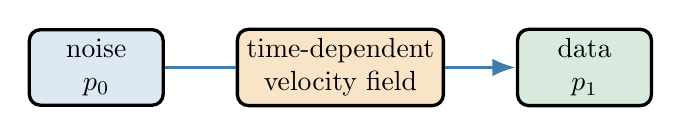
\begin{tikzpicture}[node distance=0.9cm]
    \node[box,fill=courselightblue] (base) {noise\\\(p_0\)};
    \node[box,fill=courselightorange,right=of base] (field) {time-dependent\\velocity field};
    \node[box,fill=coursegreen!18,right=of field] (data) {data\\\(p_1\)};
    \draw[flow] (base)--(field)--(data);
  \end{tikzpicture}

  \raggedright
  \vspace{0.3cm}
  \(p_0\) is the density of the starting noise (for example a Gaussian); \(p_1\) is the density of the data we want to imitate.

  \textbf{So:} a generator is a rule for moving each noise point to a data point.
\end{frame}

\begin{frame}{Time Convention (Opposite to the Diffusion Deck)}
  \begin{itemize}
    \item \textbf{This deck:} \(t=0\) is \textbf{noise}, \(t=1\) is \textbf{data}; generation runs forward from \(0\) to \(1\).
    \item \textbf{Diffusion deck:} \(t=0\) is data and \(t=T\) is noise; generation runs backward.
    \item To translate: flow time \(t\) corresponds to diffusion step \(T(1-t)\).
  \end{itemize}
  The two decks use the same ideas with the clock running in opposite directions.

  \medskip
  \textbf{So:} whenever a formula here says \(t=1\), think ``finished sample''.
\end{frame}

\begin{frame}{A Velocity Field Tells Every Point Where to Go}
  \[
    \boxed{\frac{d\mathbf x_t}{dt}=\mathbf v_t(\mathbf x_t)},\qquad t\in[0,1].
  \]
  \begin{itemize}
    \item \(\mathbf v_t(\mathbf x)\) is the \textbf{velocity field}: at time \(t\) and position \(\mathbf x\) it gives the speed and direction of motion.
    \item Like wind on a map: a leaf dropped at \(\mathbf x_0\) is carried along.
  \end{itemize}
  \textbf{Example} (1D, constant field \(v_t(x)=2\)): a point starting at \(x_0=0.5\) is at \(x_t=0.5+2t\), so at \(x_1=2.5\).

  \medskip
  \textbf{So:} given the field and a starting point, the whole path is determined.
\end{frame}

\begin{frame}{The Flow Map and the Learned Field}
  \begin{itemize}
    \item The \textbf{flow map} \(\phi_t\) records where a start point ends up: \(\mathbf x_t=\phi_t(\mathbf x_0)\).
    \item Following the field for the whole time carries every noise point to a data-like point: \(\phi_1\).
    \item We cannot write the right field by hand, so a neural network \(\mathbf v_\theta(\mathbf x,t)\) approximates it.
  \end{itemize}
  (The field must be smooth enough that each starting point has exactly one path.)

  \medskip
  \textbf{So:} learning to generate means learning a velocity field.
\end{frame}

\begin{frame}{Moving Points Change the Density}
  Let \(p_t(\mathbf x)\) be the density of the whole cloud at time \(t\).
  \begin{itemize}
    \item Where points converge, the cloud gets \textbf{denser}; where they spread out, it thins.
    \item Points are neither created nor destroyed, only moved.
  \end{itemize}
  \[
    \boxed{\partial_t p_t(\mathbf x)+\nabla_{\mathbf x}\cdot\big(p_t(\mathbf x)\,\mathbf v_t(\mathbf x)\big)=0}
  \]
  In words: the density at a place goes up exactly when more probability flows in than flows out.
  This is the \textbf{continuity equation}.

  \medskip
  \textbf{So:} choosing a velocity field is the same as choosing how the density changes in time.
\end{frame}

\begin{frame}{Recap of Part 1}
  \begin{itemize}
    \item Generating = moving noise points to data points along a velocity field.
    \item The field fixes every path and how the density changes.
    \item In this deck \(t=0\) is noise and \(t=1\) is data.
  \end{itemize}
  \textbf{Next:} how to train a network to represent a field that carries \(p_0\) to \(p_1\).
\end{frame}

\section{Learning the Velocity Field}
\sectiondivider{Part 2: Learning the Velocity Field}

\begin{frame}{The Training Goal: Regress a Target Velocity}
  Suppose we had a field \(\mathbf u_t\) that carries \(p_0\) to \(p_1\) (the \textbf{target velocity}). Train
  \[
    \boxed{L_{\mathrm{FM}}(\theta)=\mathbb E_{t,\mathbf x_t\sim p_t}\big\|\mathbf v_\theta(\mathbf x_t,t)-\mathbf u_t(\mathbf x_t)\big\|^2}.
  \]
  \begin{itemize}
    \item \(\mathbb E\): average over a random time \(t\) and a random point \(\mathbf x_t\) of the moving cloud.
    \item The target is a \emph{vector} (a direction and speed), not a noise sample or a final image.
  \end{itemize}
  \textbf{So:} it is ordinary regression, if only we knew \(\mathbf u_t\).
\end{frame}

\begin{frame}{The Problem: We Do Not Know \(\mathbf u_t\)}
  \begin{itemize}
    \item The cloud \(p_t\) in between noise and data is itself unknown.
    \item Many fields carry \(p_0\) to \(p_1\); computing even one directly is hard.
  \end{itemize}
  The fix: do not ask for the global field. Ask, for \emph{one pair} of a noise point and a data point,
  how a point would move between them. That is easy.

  \medskip
  \textbf{So:} replace one hard global question by many easy per-pair questions.
\end{frame}

\begin{frame}{Conditional Paths: Pick a Pair, Pick a Path}
  Let \(Z\) be a helper random variable that fixes one simple path (for us: a pair \(Z=(\mathbf x_0,\mathbf x_1)\)).
  \begin{itemize}
    \item \(p_t(\mathbf x\mid Z)\): where a point is at time \(t\) if it follows the path chosen by \(Z\).
    \item \(\mathbf u_t(\mathbf x\mid Z)\): its velocity, known exactly because we chose the path.
  \end{itemize}
  Train on samples: draw \(Z\), draw a time \(t\), compute the point on the path, regress onto the pair's velocity:
  \[
    L_{\mathrm{CFM}}=\mathbb E\,\|\mathbf v_\theta(\mathbf x_t,t)-\mathbf u_t(\mathbf x_t\mid Z)\|^2.
  \]
  \textbf{So:} every training example is a point on a simple path with a known velocity.
\end{frame}

\begin{frame}{Rectified Flow: The Simplest Choice Is a Straight Line}
  For a pair \((\mathbf x_0,\mathbf x_1)\) take the straight line between them:
  \[
    \boxed{\mathbf x_t=(1-t)\,\mathbf x_0+t\,\mathbf x_1},\qquad
    \frac{d\mathbf x_t}{dt}=\mathbf x_1-\mathbf x_0 .
  \]
  \textbf{Example} (1D): \(x_0=-1\), \(x_1=3\). At \(t=0.25\) the point is at \(0\); its velocity is \(3-(-1)=4\) at all times.

  \medskip
  The loss becomes \(\mathbb E\|\mathbf v_\theta(\mathbf x_t,t)-(\mathbf x_1-\mathbf x_0)\|^2\): predict the displacement.

  \textbf{So:} the training target is simply ``end minus start''.
\end{frame}

\begin{frame}{Coupling: How Noise Points Are Paired With Data Points}
  The pairing rule is a \textbf{coupling} \(\pi(\mathbf x_0,\mathbf x_1)\): a recipe for drawing pairs
  whose first parts follow \(p_0\) and second parts follow \(p_1\).
  \begin{itemize}
    \item \textbf{Independent coupling} (the default here): draw \(\mathbf x_0\) and \(\mathbf x_1\) separately.
    \item \textbf{Other couplings} (for example optimal-transport pairings) match nearby points and shorten the paths.
  \end{itemize}
  \textbf{So:} with independent pairing, a noise point is matched to a random data point, however far away.
\end{frame}

\begin{frame}{Independent Pairs Make Straight Paths That Cross}
  \centering
  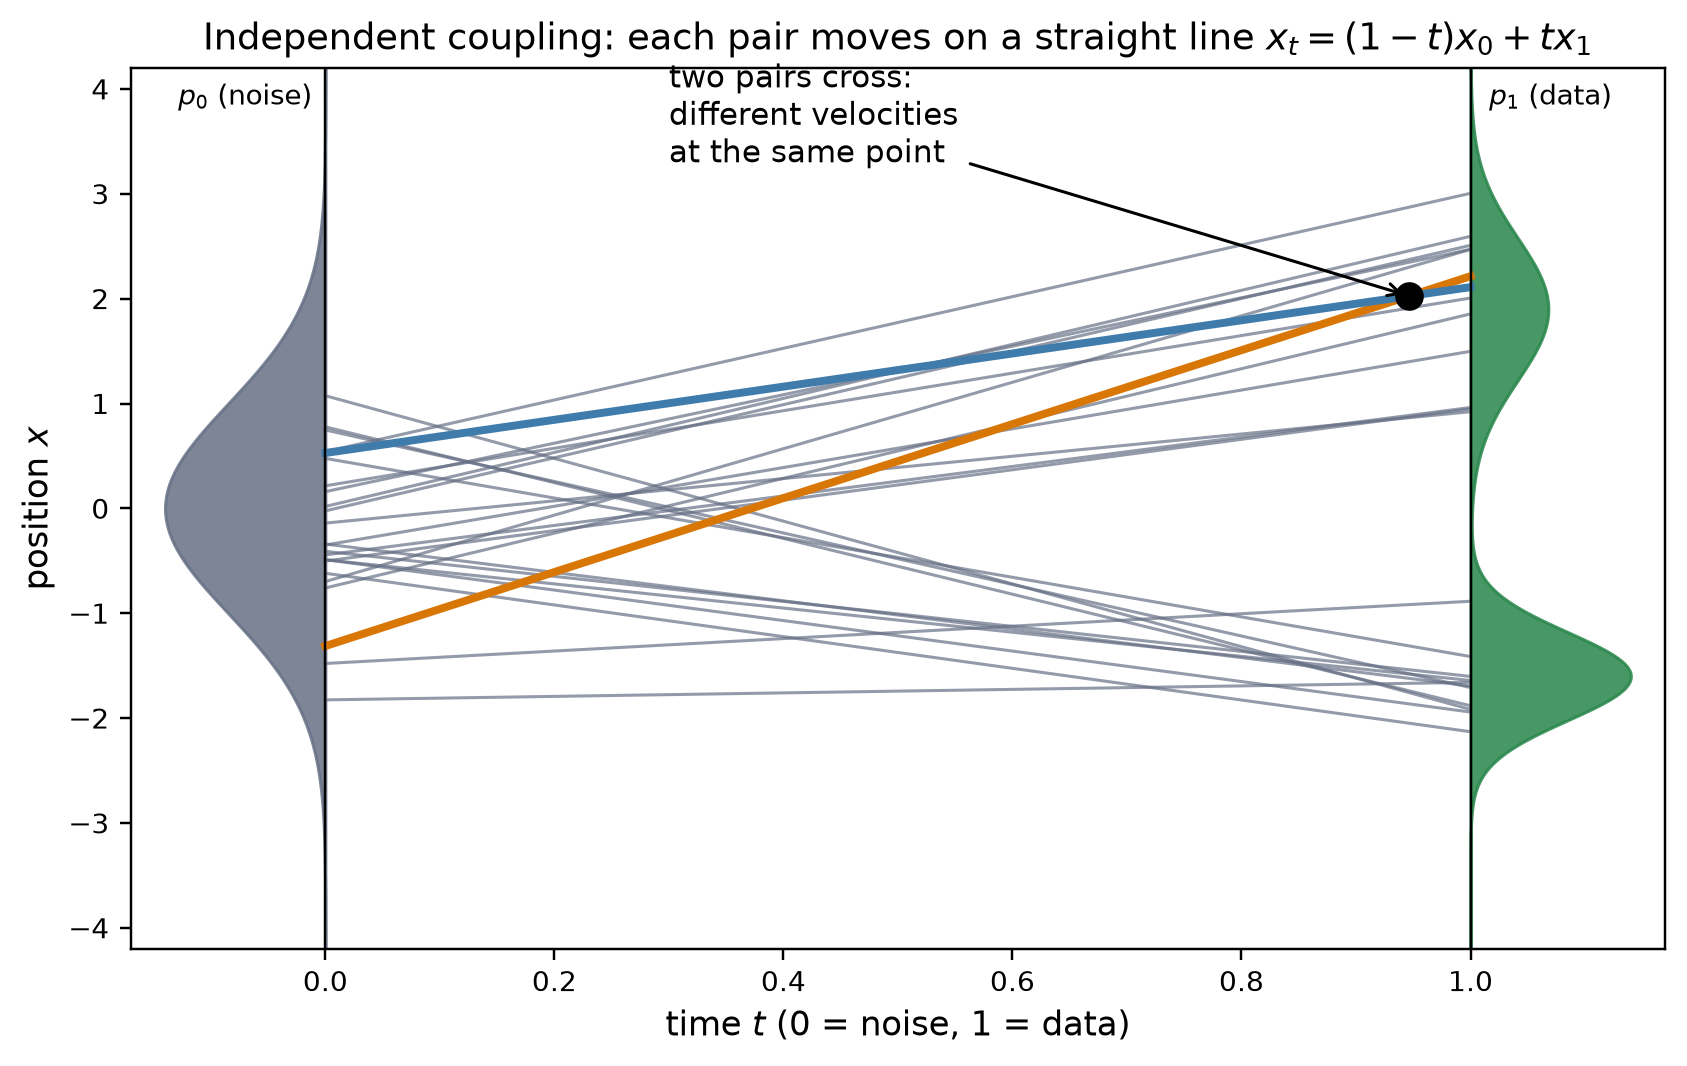
\includegraphics[width=0.85\textwidth]{flow_matching_independent_pairs.png}

  \raggedright
  \small 24 independent pairs. The orange and blue pairs pass through the same point at the same time with different velocities.

  \textbf{So:} at a crossing, the per-pair targets disagree about where to go.
\end{frame}

\begin{frame}{Regression Averages the Disagreeing Targets}
  \begin{itemize}
    \item At a crossing point, one pair says ``move \(+3\)'' and another ``move \(-1\)''.
    \item Squared error is smallest for their \emph{average}, here \(+1\) (with equal weights).
    \item In general the learned field at \((\mathbf x,t)\) is the average velocity of all pairs passing through \(\mathbf x\) at time \(t\):
      \(\mathbf u_t(\mathbf x)=\mathbb E[\mathbf x_1-\mathbf x_0\mid\mathbf x_t=\mathbf x]\).
    \item This averaged field carries \(p_0\) to \(p_1\) (details in the appendix).
  \end{itemize}
  \textbf{So:} no single pair is followed exactly; the field follows the crowd.
\end{frame}

\begin{frame}{The Averaged Field and the Paths It Creates}
  \centering
  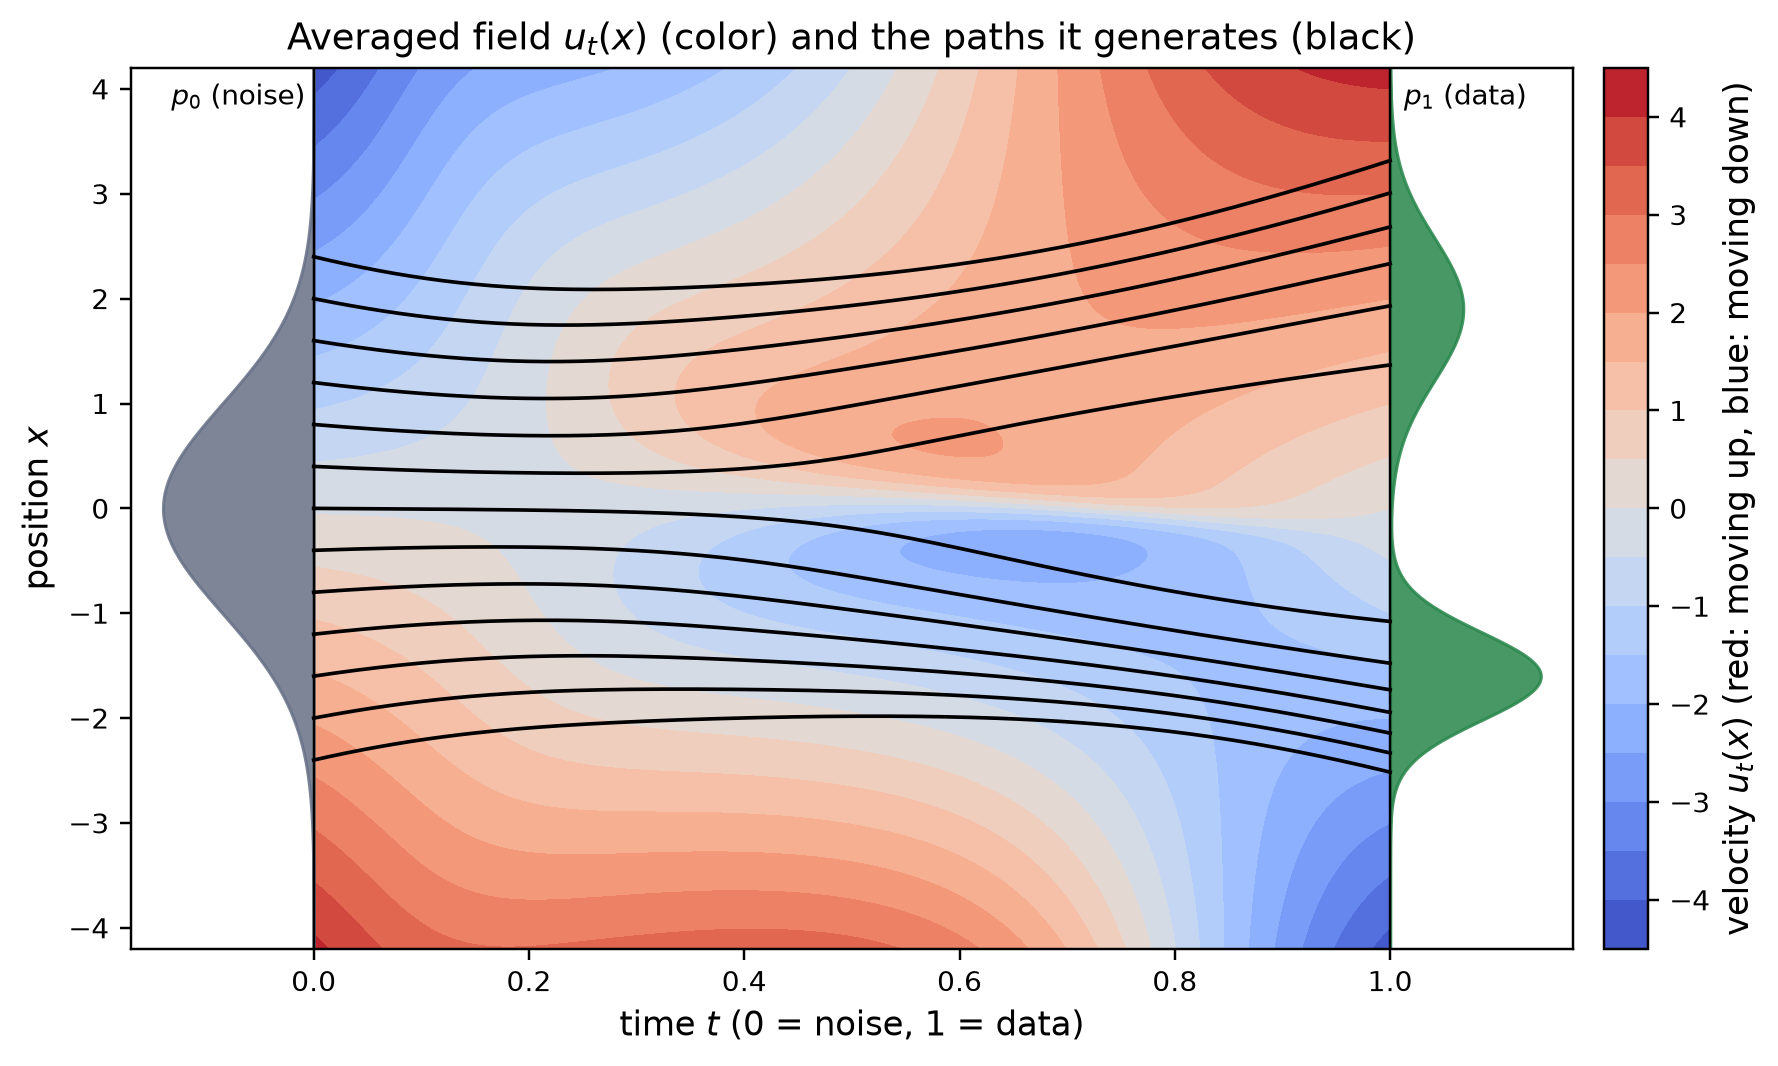
\includegraphics[width=0.85\textwidth]{flow_matching_marginal_field.png}

  \raggedright
  \small Exact averaged field for the same independent coupling (no network trained). Black curves follow the field from 13 starting points.

  \textbf{So:} the paths of the averaged field never cross and bend gently, unlike the straight pair paths.
\end{frame}

\begin{frame}{Recap of Part 2}
  \begin{itemize}
    \item Training target: a velocity; we cannot compute the global one, but we can for each pair.
    \item Rectified flow: straight line per pair, target \(\mathbf x_1-\mathbf x_0\).
    \item The coupling decides which pairs are drawn; regression averages their velocities.
  \end{itemize}
  \textbf{Next:} turn the learned field into samples by solving an ODE.
\end{frame}

\section{Sampling and Its Errors}
\sectiondivider{Part 3: Sampling and Its Errors}

\begin{frame}{Sampling: Follow the Learned Field Step by Step}
  Draw \(\mathbf x_0\sim p_0\) and solve
  \(\dfrac{d\mathbf x_t}{dt}=\mathbf v_\theta(\mathbf x_t,t)\) from \(t=0\) to \(1\).
  The simplest solver is \textbf{Euler's method}: with step \(\Delta t\),
  \[
    \mathbf x_{n+1}=\mathbf x_n+\Delta t\,\mathbf v_\theta(\mathbf x_n,t_n).
  \]
  \textbf{Example:} \(\Delta t=0.25\), four steps; at each one ask the network for the velocity and move by \(0.25\) times it.

  \medskip
  \textbf{So:} sampling needs one network evaluation per step; fewer steps are cheaper but less accurate.
\end{frame}

\begin{frame}{The Cloud Turns Into the Data Distribution}
  \centering
  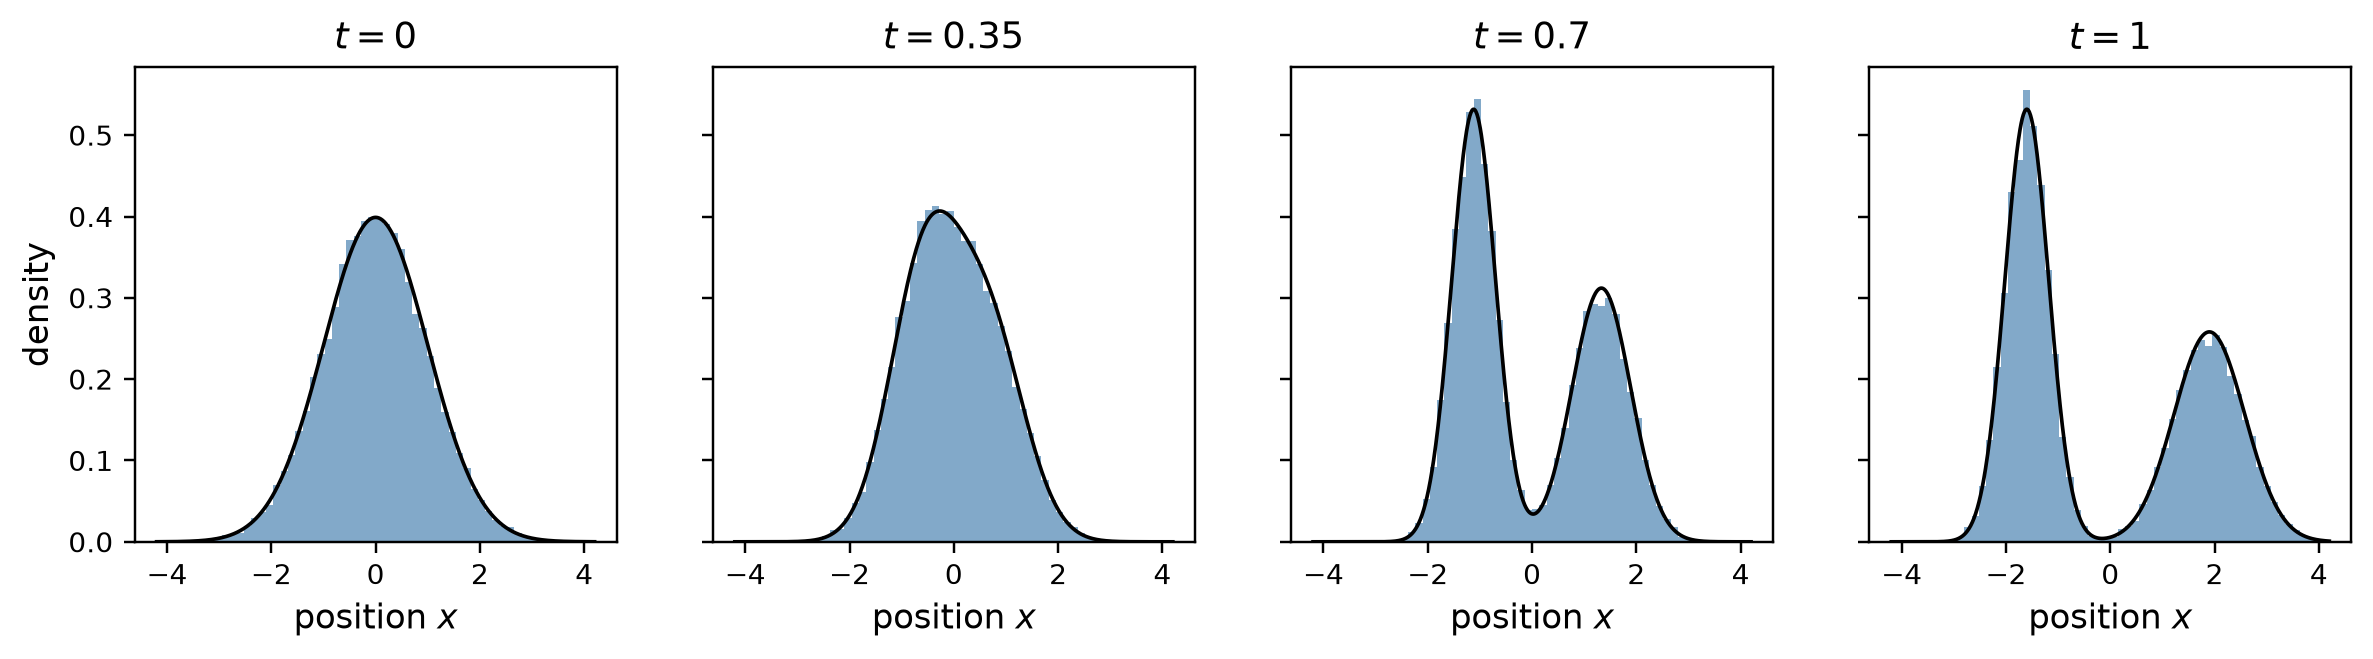
\includegraphics[width=0.98\textwidth]{flow_matching_density_evolution.png}

  \raggedright
  \small 20\,000 points start as Gaussian noise and follow the exact averaged field (200 midpoint steps). Histogram: points; black curve: exact density at that time.

  \textbf{So:} following the field really does turn noise into the two-bump data distribution.
\end{frame}

\begin{frame}{Model Error and Solver Error Are Different}
  Generation can go wrong for two separate reasons:
  \begin{itemize}
    \item \textbf{Model error:} the network field \(\mathbf v_\theta\) differs from the ideal field \(\mathbf u_t\).
    \item \textbf{Solver error:} the numerical steps differ from the exact solution of the ODE.
  \end{itemize}
  Smaller steps reduce solver error only. Better regression reduces model error only.

  \medskip
  \textbf{So:} to diagnose a bad sample, change the step count first: if it improves, it was solver error.
\end{frame}

\begin{frame}{Why Straight Paths Can Need Fewer Steps}
  \begin{itemize}
    \item Euler is \emph{exact} along a path whose velocity does not change.
    \item The more the velocity changes along a path, the smaller the steps must be.
    \item A pair's path is straight, but the averaged field's paths can still bend (previous figure), so fewer steps help only if the learned paths are nearly straight.
  \end{itemize}
  \textbf{So:} straighter learned paths allow larger steps; straightness of training pairs alone does not guarantee it.
\end{frame}

\begin{frame}{Recap of Part 3}
  \begin{itemize}
    \item Sampling = solving the learned ODE, here with Euler steps.
    \item Quality = model error plus solver error; they are checked separately.
  \end{itemize}
  \textbf{Next:} how flow matching relates to diffusion, where it is used, and its limits.
\end{frame}

\section{Context: Diffusion, Uses and Limits}
\sectiondivider{Part 4: Context, Uses and Limits}

\begin{frame}{Flow Matching and Diffusion Compared}
  \footnotesize
  \begin{center}
  \begin{tabular}{p{2.6cm}p{3.2cm}p{3.2cm}}
    \hline
      & Diffusion & Flow matching\\
    \hline
    Network predicts & noise or score & velocity\\
    Path, noise to data & fixed Gaussian corruption & any chosen path\\
    \(t=0\) means & data & noise\\
    Sampling & denoise step by step & solve an ODE\\
    Randomness & optional while sampling & only the starting noise\\
    \hline
  \end{tabular}
  \end{center}
  \normalsize
  Both learn a time-dependent vector field over intermediate states.

  \textbf{So:} same family of ideas; the difference is the path and what the network is asked to predict.
\end{frame}

\begin{frame}{A Bridge From Diffusion}
  Diffusion can also be written in continuous time as a random motion (an SDE).
  \begin{itemize}
    \item A deterministic ODE with the \emph{same} density at every time exists; its velocity is built from the learned score.
    \item So a trained diffusion model also defines a velocity field to follow.
    \item Flow matching instead regresses a velocity for a path we choose.
  \end{itemize}
  The formulas for the SDE and this ODE are in the appendix; this deck owns the continuous-time view.

  \medskip
  \textbf{So:} diffusion samplers and flow matching both move points along a velocity field.
\end{frame}

\begin{frame}{Flow Matching Supports Many Data Domains}
  \begin{itemize}
    \item images, audio and video,
    \item molecular and geometric structures,
    \item physical fields and ensembles of simulations,
    \item conditional inverse problems,
    \item generation in a learned latent space.
  \end{itemize}
  The network and the starting distribution must match the data; constraints may need equivariant fields, projection or conditioning.

  \medskip
  \textbf{So:} the method is general; the engineering is data-specific.
\end{frame}

\begin{frame}{Limitations Come From Paths, Models and Solvers}
  \begin{itemize}
    \item Poor couplings give noisy or strongly curved targets.
    \item Finite data and limited capacity bias the learned field.
    \item Outside the training distribution the learned transport is not reliable.
    \item Results can depend on solver settings.
    \item Likelihoods need extra work (appendix: divergence integral).
    \item Claims of fast sampling need matched quality and evaluation counts.
  \end{itemize}
  \textbf{So:} always report quality together with the number of network evaluations.
\end{frame}

\begin{frame}{Summary}
  \begin{itemize}
    \item A velocity field moves noise points to data points; the continuity equation tracks the density.
    \item Per-pair straight paths give simple regression targets; the learned field is their average.
    \item Sampling solves the ODE; model and solver errors are separate.
  \end{itemize}
  \textbf{So:} flow matching learns directly how to move noise into data.
\end{frame}

\appendix
\sectiondivider{Appendix: optional depth}

\begin{frame}{Pushforward Notation and the Flow of Densities}
  The flow map moves the starting density: the density of \(\phi_t(\mathbf x_0)\) is written
  \[
    p_t=(\phi_t)_\#\,p_0 \qquad(\text{``pushforward'': the density of the moved points}).
  \]
  Equivalently, for a region \(A\), \(p_t(A)=p_0(\phi_t^{-1}(A))\): the mass in \(A\) at time \(t\) equals the starting mass that flows into \(A\).
  Under standard smoothness conditions \(\phi_t\) is invertible, so one can run the flow backward.
\end{frame}

\begin{frame}{Log Density Changes Through the Divergence}
  Along one trajectory,
  \[
    \frac{d}{dt}\log p_t(\mathbf x_t)=-\nabla_{\mathbf x}\!\cdot\mathbf v_t(\mathbf x_t),
    \qquad
    \log p_1(\mathbf x_1)=\log p_0(\mathbf x_0)-\int_0^1\nabla\!\cdot\mathbf v_t(\mathbf x_t)\,dt.
  \]
  The divergence \(\nabla\!\cdot\mathbf v\) is the Jacobian trace: positive means local expansion (density drops), negative means contraction.
  The exact trace is expensive in high dimension, so stochastic trace estimators are used.
\end{frame}

\begin{frame}{The Marginal Field as a Weighted Average (Bayes Form)}
  The minimizer of the conditional regression loss is
  \[
    \mathbf v_\star(\mathbf x,t)=\mathbb E[\mathbf u_t(\mathbf x_t\mid Z)\mid\mathbf x_t=\mathbf x]
      =\frac{\int\mathbf u_t(\mathbf x\mid z)\,p_t(\mathbf x\mid z)\,p(z)\,dz}{p_t(\mathbf x)},
  \]
  \[
    p_t(\mathbf x)=\int p_t(\mathbf x\mid z)p(z)\,dz.
  \]
  This marginal velocity satisfies the continuity equation for the marginal path \(p_t\), so it carries \(p_0\) to \(p_1\).
\end{frame}

\begin{frame}{A Gaussian Conditional Path Has an Explicit Velocity}
  Take a data endpoint \(\mathbf x_1\) and noise \(\boldsymbol\epsilon\sim\mathcal N(\mathbf0,\mathbf I)\):
  \[
    \mathbf x_t=\alpha_t\mathbf x_1+\sigma_t\boldsymbol\epsilon,
  \]
  where \(\alpha_t\) is the weight on the data (rising from \(0\) at \(t=0\) to \(1\) at \(t=1\)) and \(\sigma_t\) the noise amount (falling from \(1\) to \(0\)); dots denote \(d/dt\). Then
  \[
    \mathbf u_t(\mathbf x_t\mid\mathbf x_1)=\dot\alpha_t\mathbf x_1+\frac{\dot\sigma_t}{\sigma_t}(\mathbf x_t-\alpha_t\mathbf x_1).
  \]
  Rectified flow is the special case \(\alpha_t=t\), \(\sigma_t=1-t\).
\end{frame}

\begin{frame}{Midpoint Solver}
  A second-order alternative to Euler uses the velocity at the middle of the step:
  \[
    \mathbf k_1=\mathbf v_\theta(\mathbf x_n,t_n),
  \]
  \[
    \mathbf x_{n+1}=\mathbf x_n+\Delta t\,\mathbf v_\theta\!\big(\mathbf x_n+\tfrac{\Delta t}{2}\mathbf k_1,\;t_n+\tfrac{\Delta t}{2}\big).
  \]
  It costs two network evaluations per step and is more accurate for the same step size
  (the density figure in the main text uses it).
\end{frame}

\begin{frame}{Continuous-Time Diffusion: the SDE and the Probability-Flow ODE}
  \textbf{Convention here:} diffusion time (\(t=0\) data, \(t=T\) noise), opposite to the main text.
  A forward stochastic differential equation, with drift \(\mathbf f\), noise strength \(g(t)\) and Brownian motion \(\mathbf W_t\), is
  \[
    d\mathbf x=\mathbf f(\mathbf x,t)\,dt+g(t)\,d\mathbf W_t .
  \]
  Its reverse-time SDE and the deterministic probability-flow ODE with the same marginals \(p_t\) are
  \[
    d\mathbf x=\big[\mathbf f-g^2\nabla_{\mathbf x}\log p_t\big]dt+g\,d\overline{\mathbf W}_t,
    \qquad
    \frac{d\mathbf x}{dt}=\mathbf f(\mathbf x,t)-\tfrac12g(t)^2\nabla_{\mathbf x}\log p_t(\mathbf x).
  \]
  Individual paths differ between the two; the learned score supplies the unknown term.
\end{frame}

\end{document}
